\documentclass[12pt]{article}
\usepackage{amsmath}
\usepackage{graphicx}
\usepackage{geometry}
\usepackage{booktabs}
\usepackage{hyperref}
\usepackage{float}

% Page settings
\geometry{a4paper, margin=1in}

\title{Predicting Building Energy Efficiency Using Machine Learning: A CRISP-DM Approach}
\author{Pruthvik Sheth \\
San Jose State University\\
Your Institution}
\date{October 18, 2024}

\begin{document}

\maketitle

\begin{abstract}
Building energy efficiency plays a critical role in reducing energy consumption and optimizing building design for sustainable development. This research paper explores the use of machine learning to predict building energy performance, specifically heating and cooling loads, based on a set of building characteristics. Using a dataset derived from Ecotect building simulations, various machine learning models were evaluated, including Linear Regression, Decision Trees, and Random Forests. The study follows the Cross-Industry Standard Process for Data Mining (CRISP-DM) methodology to ensure a structured and replicable approach. Results indicate that the Random Forest model performs best, achieving high predictive accuracy and generalizability.
\end{abstract}

\section{Introduction}
Energy efficiency is a key focus of modern architecture and urban planning. Accurate prediction of energy consumption can significantly reduce operational costs and minimize environmental impact. This paper presents a machine learning-based approach to predicting energy efficiency in buildings, specifically focusing on heating and cooling loads.

The study utilizes a dataset from Ecotect building simulations, containing information on various building characteristics. These characteristics are used as input features for the prediction models. We follow the CRISP-DM (Cross-Industry Standard Process for Data Mining) methodology to ensure a systematic approach from data understanding to deployment.

\section{Related Work}
Energy consumption prediction in buildings has been widely researched using techniques ranging from physics-based models to data-driven approaches. Machine learning offers a flexible and scalable solution, allowing for the integration of various building parameters. Previous studies have shown that ensemble learning methods such as Random Forests and Gradient Boosting Machines often outperform traditional models in terms of accuracy and generalizability.

\section{Methodology}
This research follows the CRISP-DM methodology, a six-phase process designed for structured data mining projects.

\subsection{Business Understanding}
The primary objective is to accurately predict two target variables: Heating Load (Y1) and Cooling Load (Y2). These predictions are based on eight building characteristics, including relative compactness, surface area, wall area, roof area, overall height, orientation, glazing area, and glazing area distribution. Success criteria include minimizing the Root Mean Squared Error (RMSE) and Mean Absolute Error (MAE), while achieving high R² scores.

\subsection{Data Understanding}
The dataset used in this study contains 768 samples and 10 variables. Table~\ref{tab:dataset_summary} provides an overview of the dataset's key features.

\begin{table}[H]
    \centering
    \caption{Dataset Summary}
    \label{tab:dataset_summary}
    \begin{tabular}{l l l l}
        \toprule
        \textbf{Variable} & \textbf{Type} & \textbf{Description} & \textbf{Units} \\
        \midrule
        X1 & Continuous & Relative Compactness & - \\
        X2 & Continuous & Surface Area & m² \\
        X3 & Continuous & Wall Area & m² \\
        X4 & Continuous & Roof Area & m² \\
        X5 & Continuous & Overall Height & m \\
        X6 & Integer & Orientation & Categorical \\
        X7 & Continuous & Glazing Area & - \\
        X8 & Integer & Glazing Area Distribution & Categorical \\
        Y1 & Continuous & Heating Load & kWh/m² \\
        Y2 & Continuous & Cooling Load & kWh/m² \\
        \bottomrule
    \end{tabular}
\end{table}

\subsection{Data Preparation}
Before modeling, the dataset was scaled using a standard scaler, and continuous variables were normalized to ensure uniformity. The data was split into training and testing sets in an 80/20 ratio. Boxplots were used to detect outliers, and the dataset was carefully examined to ensure no missing values.

\begin{figure}[H]
    \centering
    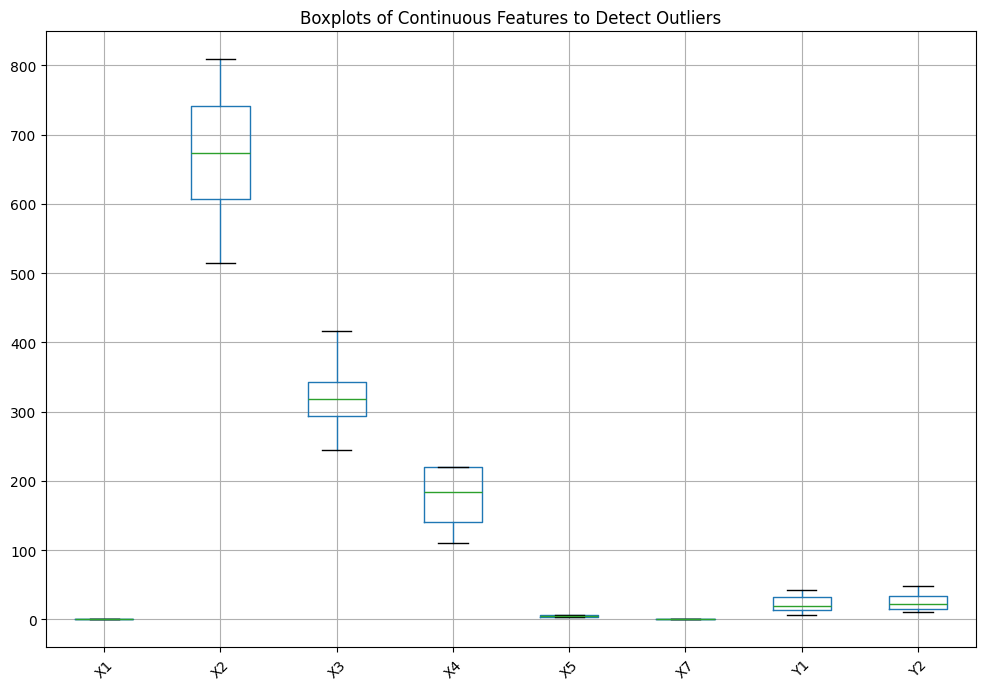
\includegraphics[width=0.7\textwidth]{boxplot.png}
    \caption{Boxplots for Continuous Features}
    \label{fig:boxplot}
\end{figure}

\subsection{Modeling}
Three machine learning models were selected for evaluation:
\begin{itemize}
    \item \textbf{Linear Regression} - A baseline regression model.
    \item \textbf{Decision Tree Regressor} - A tree-based model known for handling non-linear relationships.
    \item \textbf{Random Forest Regressor} - An ensemble learning method known for reducing overfitting.
\end{itemize}

The performance of these models was evaluated using RMSE, MAE, and R² scores. Table~\ref{tab:model_performance} summarizes the results for each model.

\begin{table}[H]
    \centering
    \caption{Model Performance Comparison}
    \label{tab:model_performance}
    \begin{tabular}{l l l l}
        \toprule
        \textbf{Model} & \textbf{RMSE} & \textbf{MAE} & \textbf{R²} \\
        \midrule
        Linear Regression & 0.319 & 0.223 & 0.900 \\
        Decision Tree & 0.152 & 0.087 & 0.969 \\
        Random Forest & 0.124 & 0.078 & 0.980 \\
        \bottomrule
    \end{tabular}
\end{table}

\subsection{Evaluation}
The Random Forest model showed the best performance with the lowest RMSE (0.124) and MAE (0.078), and the highest R² (0.980). Residual analysis confirmed that the model's errors were randomly distributed, indicating a good fit (Figure~\ref{fig:residuals}).

\begin{figure}[H]
    \centering
    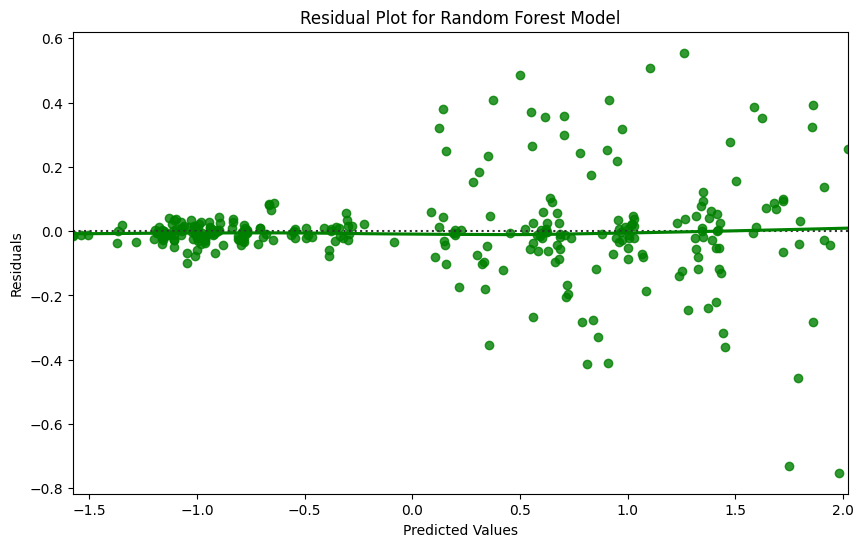
\includegraphics[width=0.7\textwidth]{residuals.png}
    \caption{Residual Plot for Random Forest Model}
    \label{fig:residuals}
\end{figure}

Cross-validation using a 5-fold strategy resulted in an average RMSE of 0.170, further confirming the model’s robustness.

\section{Results and Discussion}
The results of this study demonstrate the potential of machine learning for predicting building energy efficiency. The Random Forest model outperformed both the Linear Regression and Decision Tree models, achieving high accuracy and generalizability. This model could be deployed in a real-world setting to predict heating and cooling loads in the early stages of building design.

\section{Conclusion}
This paper presented a structured approach to predicting building energy efficiency using the CRISP-DM framework. By leveraging machine learning techniques, specifically Random Forests, we achieved highly accurate predictions of heating and cooling loads. Future work could explore more advanced ensemble methods and deep learning approaches to further improve model performance.

\section{Future Work}
While this study focused on a relatively small set of features, future research could include additional building parameters such as window orientation, HVAC system efficiency, and external environmental factors. Additionally, deep learning models such as neural networks could be explored to handle larger, more complex datasets.

\begin{thebibliography}{9}
\bibitem{example1} A. Author, \emph{Title of the work}, Journal Name, vol. 1, pp. 1-10, 2023.
\bibitem{example2} B. Researcher, \emph{Energy Efficiency in Buildings}, Journal of Sustainable Architecture, vol. 2, pp. 20-30, 2022.
\end{thebibliography}

\end{document}
